\documentclass[blue]{ludusofficial}

\usepackage{amsmath}
\usepackage[hyphens]{url}
\usepackage{dblfloatfix}
\usepackage{placeins}
\usepackage{booktabs}
\usepackage{lineno}
\linenumbers
\usepackage{setspace}

\setcounter{topnumber}{4}
\setcounter{dbltopnumber}{4}
\renewcommand{\topfraction}{0.95}
\renewcommand{\dbltopfraction}{0.95}
\renewcommand{\textfraction}{0.05}

\title{How the Follow-up Definition Creates Prognostic Value in Longitudinal MRI:\\[8pt]A Landmark Analysis of Cortical Boundary Sharpness in Mild Cognitive Impairment}

\shorttitle{Follow-up Definition and Longitudinal MRI Prediction}
\shortauthor{Cherukuri}

\author{%
    \textbf{Ishaan Cherukuri}\textsuperscript{1}\textsuperscript{*}\\[0.2cm]
    \small\textsuperscript{1}Independent Researcher, USA\\
    \small Corresponding: ishaan.cherukuri@gmail.com\\[0.4cm]
    \small\textsuperscript{*}Data used in preparation of this article were obtained from the Alzheimer's Disease Neuroimaging Initiative (ADNI) database (adni.loni.usc.edu). The investigators within ADNI contributed to the design and implementation of ADNI and provided data but did not participate in the analysis or writing of this report. A complete listing of ADNI investigators is available at: \href{http://adni.loni.usc.edu/wp-content/uploads/how_to_apply/ADNI_Acknowledgement_List.pdf}{adni.loni.usc.edu/how\_to\_apply/ADNI\_Acknowledgement\_List.pdf}
}

\begin{document}

\begin{abstract}
Machine learning models built on longitudinal MRI routinely report strong prediction of conversion from mild cognitive impairment to Alzheimer's disease. This study asks how much of that performance comes from the imaging and how much from how follow-up time is defined. Cortical boundary sharpness, a T1-derived measure of how sharply grey and white matter separate, serves as the test case, because its rate of change has been proposed as an early marker of cortical degeneration and because it is measured on the same scans that supply conventional morphometry. Boundary sharpness maps and morphometry were computed for 3{,}720 T1-weighted scans from 657 ADNI participants. Two survival designs were compared on the same participants, features, folds and random seed. In the first, the survival clock starts at the baseline scan while features are drawn from the entire scan series, which is the design used in much of this literature. In the second, a landmark design, features come only from scans acquired while the participant was still cognitively impaired without dementia, participants who converted before the landmark are excluded, and follow-up starts at the landmark. Changing only the clock moved boundary sharpness slopes from a cross-validated C-index of 0.720 to 0.501 and combined imaging from 0.672 to 0.534, while a model of age, sex, education and Mini-Mental State Examination score was unaffected and rose from 0.684 to 0.747. Under the landmark design, clinical variables alone reached 0.747 $\pm$ 0.024 across folds, boundary sharpness slopes reached 0.556 and morphometry 0.587. Adding the boundary block to clinical variables changed discrimination by 0.000 (95\% confidence interval $-0.013$ to $+0.013$) and did not improve Cox partial likelihood ($\chi^2 = 5.1$, 20 degrees of freedom, $P = 1.00$). To test whether a short observation window explained the null, the landmark was swept from 12 to 48 months, quadrupling the mean pre-landmark window from 0.81 to 3.04 years. The increment remained on zero at every window and no slope survived false discovery correction at any of them. Boundary sharpness magnitude differed by scanner field strength ($d = 0.30$) and tracked signal-to-noise ratio ($r = 0.22$), both larger than any difference between participants who converted and those who did not. Reported prognostic value here is a property of the study design rather than of the images.
\end{abstract}

\keywords{Alzheimer's disease; mild cognitive impairment; landmark analysis; guarantee-time bias; immortal time bias; survival analysis; longitudinal MRI; boundary sharpness coefficient; incremental prognostic value; prediction model; ADNI}

\maketitle

\doublespacing

\section{Introduction}

Around 10 to 15 per cent of people with mild cognitive impairment (MCI) progress to dementia each year, and the average conceals a wide range of individual trajectories. Some people remain stable for a decade, some revert to normal cognition, and some decline quickly. Anti-amyloid therapies such as lecanemab and donanemab are indicated for early disease, which has made the question of who will progress, and when, a practical one rather than an academic one.

Structural MRI is attractive for that question because it is already part of a standard cognitive workup, costs a fraction of amyloid PET, and requires no lumbar puncture. Cross-sectional MRI markers have generally disappointed, which motivated a shift toward longitudinal features: rather than asking how atrophied a brain is today, ask how fast it is changing. Rates of change should in principle carry information that a single scan cannot.

Reported performance for such models is often high. Systematic reviews of machine learning for MCI progression report cross-validated areas under the curve near 0.78 for cognitive testing alone, comparable figures for MRI alone, and higher values for combinations \cite{ansart2021predicting, grueso2021machine}. The same reviews note that reported performance depends strongly on design choices, that studies using a single train and test split report higher numbers than cross-validated ones, and that most studies treat conversion as a binary label inside a fixed horizon rather than as a time-to-event outcome. A recent systematic review of multivariable models for MCI to dementia conversion found limited generalizability and a high risk of bias across the published literature \cite{vermeulen2025review}.

One design choice has received less attention than it deserves, and it concerns where the survival clock starts. A typical longitudinal pipeline identifies participants who were MCI at a baseline scan, computes features from each participant's series of scans, and models time from the baseline scan to the conversion visit. That arrangement has two problems that both inflate apparent performance.

The first is direct outcome leakage. If a participant converted at month 24 and was scanned at months 0, 12, 24 and 36, then two of the four scans used to build their features were acquired after the diagnosis the model is asked to predict. The model is not forecasting an event, it is recognising one that has already happened.

The second is subtler and is a form of guarantee-time bias \cite{anderson1983analysis, giobbie2013guarantee}. A participant contributes four scans only if they remained enrolled long enough to be scanned four times. Any feature that summarises variability across a participant's scan series therefore encodes how long they stayed in the study, which is closely related to how long they survived without a diagnosis. Features that look anatomical, such as the standard deviation of brain volume across a series, can behave as proxies for follow-up duration.

The consequence is that a model can score well on a concordance index without carrying prognostic information. Discrimination that arises this way does not transfer, because it depends on a cohort's scheduling conventions rather than on biology.

This study measures the size of that effect directly and asks what remains once it is removed. The test case is the boundary sharpness coefficient (BSC), a measure of how rapidly image intensity changes across the grey and white matter interface \cite{olafson2021bsc}. BSC is a useful probe for three reasons. Intracortical myelin and the sharpness of the cortical boundary are plausible early targets in neurodegeneration, so a longitudinal BSC measure has a defensible biological rationale. It is computed from the same T1-weighted scans that supply conventional morphometry, so the two can be compared on identical images without any additional acquisition. And it has no established prognostic literature to defend, which makes it a fair vehicle for a methodological question.

Three questions are addressed. First, how much cross-validated discrimination is attributable to the follow-up definition, holding participants, features, folds and seed fixed. Second, what incremental value longitudinal BSC and conventional morphometry retain over age, sex, education and Mini-Mental State Examination (MMSE) score once the design is corrected. Third, whether any apparent null is explained by a short observation window, which is tested by sweeping the landmark from 12 to 48 months.

\section{Materials and methods}

\subsection{Participants and imaging data}

Data came from the Alzheimer's Disease Neuroimaging Initiative. ADNI was launched in 2003 as a public and private partnership led by Michael W. Weiner. Its goal has been to test whether serial MRI, PET, other biological markers, and clinical and neuropsychological assessment can measure the progression of MCI and early Alzheimer's disease.

T1-weighted scans were drawn from BIDS-converted ADNI 1, GO, 2, 3 and 4 archives, giving 3{,}720 scans across 657 participants who were classified as MCI at their first scan and had a clinical diagnostic record. Diagnosis and visit dates came from the ADNIMERGE2 DXSUM table rather than from the diagnosis attached to a scan. This matters for the landmark design described below: censoring a participant at their last MRI leaves every non-converter with no follow-up after the landmark, which would remove the comparison group entirely.

Preprocessing used N4 bias correction \cite{tustison2010n4}, brain extraction with SynthStrip \cite{hoopes2022synthstrip}, and three-tissue segmentation with Atropos \cite{avants2011atropos}, all applied identically to every scan.

\subsection{Boundary sharpness and morphometry}

BSC was computed voxel-wise at the grey and white matter interface as the component of the intensity gradient aligned with the tissue-probability normal, smoothed at 1\,mm. Summaries retained per scan were the number of boundary voxels, mean and 90th percentile gradient magnitude, mean gradient direction, and the same quantities within eight spatial bins that preserve coarse topography. Annualised slopes were fitted by ordinary least squares against scan date within a participant's window, giving 20 BSC slope features after fold-internal selection.

The pipeline segments tissue probabilistically and does not construct a cortical surface, so there is no parcellation to project onto without adding a registration step and its own failure modes to every scan. With 160 events in the primary cohort, moving from global and coarse-bin summaries to several hundred correlated regional coefficients would also worsen an events-per-predictor ratio that is already 1.9 for the largest feature set used here. The eight spatial bins are a compromise that keeps some topography at a fraction of the parameter cost.

Conventional morphometry was extracted from the same segmentations: total brain volume, brain parenchymal fraction, grey matter, white matter and cerebrospinal fluid volumes, total intracranial volume, mean brain intensity, and signal-to-noise ratio. Each quantity was summarised cross-sectionally at the first scan in the window and as a trajectory across the window, giving 60 morphometry features.

Clinical covariates were age at the landmark, sex, years of education, and MMSE from the clinical visit closest to the landmark within one year. MMSE was missing for 21 of 557 participants in the primary cohort and was imputed to the training-fold median inside each fold.

\subsection{Two follow-up definitions}

The \textit{baseline-anchored} design is the one common in this literature and is reproduced here for comparison. Features are computed from every scan a participant contributed. The survival clock starts at the first scan and runs to the conversion visit, or to the last scan for non-converters.

The \textit{landmark} design places a landmark $L$ months after the first MCI scan, with a 90-day grace period for visit scheduling. Three rules follow. Only scans acquired at or before the landmark contribute to any feature. Participants who converted at or before the landmark are excluded rather than counted as events, since they are no longer at risk. Follow-up runs from the landmark to the first clinical visit with a dementia diagnosis, or to the last clinical visit for non-converters. Participants with fewer than two scans in the window, which would leave a slope unidentified, were excluded.

The primary analysis places the landmark at 24 months. To test whether the null result depends on that choice, the landmark was also placed at 12, 36 and 48 months, and every cohort was rebuilt and every model refitted at each.

\subsection{Models and evaluation}

Six model families were fitted to each feature block: penalized Cox regression with an elastic net penalty ($\ell_1$ ratio 0.5 over a 50-point path), Weibull, log-normal and log-logistic accelerated failure time models, random survival forest \cite{ishwaran2008rsf}, and gradient boosting with an accelerated failure time objective \cite{chen2016xgboost, barnwal2022survivalxgb}.

Evaluation was 5-fold cross-validation stratified by event status. Feature selection, imputation, winsorization and scaling were fitted inside training folds only. Every model returns a risk score defined so that a larger value means earlier conversion before any metric is computed, so a concordance index below 0.5 reflects a real failure to rank rather than a sign convention. Discrimination was measured with Uno's C-index \cite{uno2011cstat}.

Because differences between feature blocks are small relative to variation between folds, block comparisons were made within folds. Both feature sets were fitted on the same training partition and scored on the same held-out participants, and the paired difference is reported with a bootstrap 95\% confidence interval and a paired $t$ test. A likelihood ratio test compared a Cox model of covariates plus BSC slopes against covariates alone. Univariate differences between participants who converted and those who did not were tested with Welch's $t$ test and corrected with the Benjamini-Hochberg procedure \cite{benjamini1995controlling}.

\subsection{Acquisition dependence}

BSC is a derivative of image intensity and should be expected to depend on acquisition. Baseline BSC magnitude was compared between 1.5\,T and 3\,T scans and correlated with signal-to-noise ratio, and the same comparisons were made for the annualised slope. A units error was found and corrected during this analysis: a subset of DICOM headers reported field strength as 15000 rather than 1.5.

\section{Results}

\subsection{Cohort}

At the 24-month landmark, 557 participants met the criteria, of whom 160 converted to dementia and 397 did not. The accounting from the 1{,}604 participants with usable scans was: 421 not MCI at their first scan, 219 converted at or before the landmark, 249 with fewer than two scans in the window, and 158 with no follow-up after the landmark. Median follow-up from the landmark was 2.5 years and participants contributed a mean of 3.6 scans across a mean window of 1.65 years. Characteristics appear in Table~\ref{tab:cohort}.

Participants who converted were older (76.6 versus 74.0 years, $d = 0.37$) and scored lower on MMSE at the landmark (26.3 versus 28.1, $d = -0.71$). No BSC slope differed between the groups after false discovery correction; the largest effect size for any slope was $d = 0.15$.

\subsection{Clinical variables outperform both imaging blocks}

Age, sex, education and MMSE at the landmark reached a cross-validated test C-index of 0.747 $\pm$ 0.024 with a training value of 0.746, a gap of essentially zero. BSC slopes reached 0.556 $\pm$ 0.045 and morphometry 0.587 $\pm$ 0.038. Combining the two imaging blocks did not help, at 0.577 $\pm$ 0.044 (Table~\ref{tab:models}).

The training and test values are as informative as the test values alone. Random survival forest fitted BSC slopes at 0.844 in training and 0.501 in testing, a gap of 0.342. Gradient boosting on the full imaging matrix fitted at 0.990 and tested at 0.534, a gap of 0.456. The clinical model has no such gap. Flexible models find structure in these imaging features that does not generalise to held-out participants.

\subsection{Incremental value is indistinguishable from zero}

Adding BSC slopes to the clinical model changed cross-validated discrimination by $-0.000$ (95\% confidence interval $-0.013$ to $+0.013$, paired $P = 0.98$). Adding both imaging blocks gave 0.737 $\pm$ 0.031 against 0.747 for covariates alone. In a Cox model, the 20 BSC slopes did not improve partial likelihood over covariates ($\chi^2 = 5.08$, 20 degrees of freedom, $P = 1.00$). Scaled Schoenfeld residuals gave no evidence against proportional hazards (minimum $P = 0.28$). In the adjusted model, MMSE carried a hazard ratio of 0.62 per standard deviation ($P = 1.2 \times 10^{-18}$) and age 1.27 ($P = 3.6 \times 10^{-4}$), and no BSC slope approached significance. Risk tertiles from the clinical model separated clearly, and adding imaging did not change the separation (Figure~\ref{fig:km}).

\subsection{The follow-up definition accounts for the earlier result}

Scoring the same 557 participants under both designs, with features, folds, hyperparameters and seed held fixed, isolates the effect of the survival clock (Figure~\ref{fig:design}).

Under the baseline-anchored definition, BSC slopes reached 0.720 and combined imaging 0.672. Under the landmark definition the same features on the same participants gave 0.501 and 0.534. Morphometry moved from 0.712 to 0.587. The clinical model moved in the opposite direction, from 0.684 to 0.747, because demographic and cognitive variables do not depend on when scans were acquired and benefit from the cleaner event times.

Feature importances under the baseline-anchored design point to the mechanism. The three largest contributors were standard deviations of image-derived quantities across a participant's scan series: background ratio (15.8 per cent of gain), brain volume (10.0 per cent) and signal-to-noise ratio (9.3 per cent). Together they account for roughly 35 per cent of the model. These quantities depend on how many scans a participant received and how regularly, which is a property of study scheduling and of remaining enrolled, not of tissue.

\subsection{A longer observation window does not recover the signal}

A natural objection is that 1.65 years and 3.6 scans are too little to estimate a degradation rate, and that the null reflects measurement noise rather than absent biology. Sweeping the landmark tests this directly (Table~\ref{tab:window}, Figure~\ref{fig:window}).

Moving the landmark from 12 to 48 months increased the mean pre-landmark window from 0.81 to 3.04 years and the mean number of scans from 2.7 to 4.6, while the cohort fell from 693 participants and 242 events to 308 and 66. The fold-matched increment of BSC slopes over clinical covariates was $+0.005$ ($-0.005$ to $+0.013$) at 12 months, $-0.000$ ($-0.013$ to $+0.013$) at 24, $-0.001$ ($-0.005$ to $+0.002$) at 36, and $-0.051$ ($-0.087$ to $-0.014$) at 48. The Cox likelihood ratio test for the BSC block gave $P = 0.96$, 1.00, 1.00 and 1.00. No BSC slope survived false discovery correction at any landmark.

Morphometry behaved the same way, reaching 0.624, 0.587, 0.592 and 0.527 across the four windows. Clinical performance rose from 0.743 to 0.796, so later landmarks select a cohort that is easier rather than harder to discriminate. If a longer window helped imaging, that trend would amplify the effect rather than mask it.

One comparison at the 12-month landmark reached nominal significance: adding BSC to covariates plus morphometry gave $+0.006$ (95\% confidence interval $+0.003$ to $+0.009$, $P = 0.03$). It is reported for completeness and should not be read as a finding. It is one of six comparisons at that landmark, the effect is 0.006 in C-index, the likelihood ratio test at the same landmark gives $P = 0.96$, no slope survives correction, and the same comparison is negative at all three longer windows.

\subsection{BSC depends more on acquisition than on conversion}

Mean baseline BSC magnitude differed between field strengths (0.639 at 1.5\,T versus 0.590 at 3\,T, $d = 0.30$, $P = 0.003$) and correlated with signal-to-noise ratio ($r = 0.22$, $P = 1.8 \times 10^{-7}$). The annualised slope also differed by field strength ($P = 0.029$). Both acquisition effects exceed the largest difference between converters and non-converters for any BSC feature in the same cohort, which was $d = 0.15$. Field strength changed during the window for 4.3 per cent of participants, which is small enough not to drive results here but would matter in a cohort with more scanner turnover.

\section{Discussion}

Longitudinal boundary sharpness carried no prognostic information about conversion from MCI to dementia beyond four routinely collected clinical variables. The increment was 0.000 in C-index with a confidence interval of roughly one hundredth in each direction, the Cox likelihood ratio test was flat, and no individual slope survived correction. The result held across six model families, across four landmark definitions spanning a fourfold range of observation window, and with conventional morphometry included or excluded.

The more useful result concerns where an earlier positive finding came from. Holding participants, features, folds and seed fixed and changing only the definition of follow-up moved boundary sharpness from 0.720 to 0.501. That is not a small correction. It is the difference between a marker that looks clinically promising and one that ranks no better than chance. Since demographic and cognitive variables were untouched by the same change, the movement cannot be attributed to cohort composition or to the metric.

This has a specific implication for how longitudinal imaging studies should be read. When features are drawn from a participant's full scan series while the clock starts at baseline, two things happen at once. Scans acquired after the outcome enter the feature set, and summary statistics across the series encode how long a participant stayed under observation. Both inflate concordance without any prognostic content. Any study that reports strong discrimination from longitudinal MRI while starting follow-up at baseline should be expected to lose much of that discrimination under a landmark design, and the magnitude here suggests the loss can be most of it.

The finding that conventional morphometry is also flat, at 0.587, deserves emphasis rather than a footnote. Brain volume and parenchymal fraction trajectories are established markers of neurodegeneration and ought to outperform this. That they do not, under a corrected design and inside a two-year window, suggests the limitation is shared across imaging trajectories rather than specific to boundary sharpness. The window sweep argues against a simple power explanation, since extending the window fourfold did not help either block.

The acquisition results give a mechanism for why a derivative-based cortical measure is fragile in a multi-site cohort. BSC magnitude varies with field strength and tracks signal-to-noise ratio more strongly than it distinguishes people who converted from people who did not. In a study where scanner platforms turn over during follow-up, an apparent slope can reflect a change of hardware rather than a change of tissue. Prospective work using this class of measure should harmonise before modelling, with ComBat-style methods or an equivalent \cite{fortin2018harmonization}, rather than adjusting for site after the fact.

Several limitations apply. The cohort is ADNI, a research sample with regular scheduling, high education and mostly white participants, so absolute performance should not be read as a clinical estimate. The landmark design costs statistical power: 219 participants who converted within 24 months were excluded because they were no longer at risk, and the 48-month landmark retains only 66 events and should be treated as descriptive. BSC was summarised globally and in eight coarse spatial bins rather than regionally, and a regional analysis with a cohort sized for it remains possible and is a different study. Conversion was defined from clinical diagnosis codes, which are interval-censored between visits \cite{zhang2024interval}, and this analysis treats event times as right-censored at the recorded visit. Finally, no external cohort was analysed under the landmark design here. Per-scan features for an independent sample were not available at the necessary granularity, and since the internal analysis finds no signal to transfer, an external test would carry little information. A landmark-consistent replication remains the appropriate next step for anyone reporting a positive result with this class of feature.

A negative result about one imaging measure is of modest interest on its own. The design effect is not. Reported prognostic value in this literature is sensitive to a modelling choice that is rarely stated explicitly and that can be checked in an afternoon by refitting under a landmark. The experiment reported here is inexpensive, applies to any longitudinal imaging marker, and is worth running before a marker is described as prognostic.

\section*{Data availability}

ADNI data are available to qualified investigators at adni.loni.usc.edu. Analysis code for the landmark cohort construction, the model ladder, the window sweep and the figures is available from the author on request.

\section*{Acknowledgements}

Data collection and sharing for this project was funded by the Alzheimer's Disease Neuroimaging Initiative (National Institutes of Health Grant U01 AG024904) and DOD ADNI (Department of Defense award number W81XWH-12-2-0012). Segmentation and boundary sharpness computation were performed on the Trillium cluster at SciNet, University of Toronto, through the Digital Research Alliance of Canada.

\section*{Funding}

No specific funding was received for this work.

\section*{Competing interests}

The author reports no competing interests.

\bibliographystyle{plain}
\bibliography{references}

\clearpage

\begin{table}[t]
\centering
\caption{Cohort characteristics at the 24-month landmark. Values are mean $\pm$ standard deviation unless noted.}
\label{tab:cohort}
\small
\begin{tabular}{lccc}
\toprule
 & All (n=557) & Converted (n=160) & Stable (n=397) \\
\midrule
Age at landmark (years)      & 74.8 $\pm$ 7.4 & 76.6 $\pm$ 6.8 & 74.0 $\pm$ 7.5 \\
Female, n (\%)               & 234 (42.0)     & 66 (41.2)      & 168 (42.3) \\
Education (years)            & 16.2 $\pm$ 2.7 & 16.1 $\pm$ 2.7 & 16.2 $\pm$ 2.7 \\
MMSE at landmark             & 27.6 $\pm$ 2.5 & 26.3 $\pm$ 2.7 & 28.1 $\pm$ 2.2 \\
Scans in window              & 3.6 $\pm$ 0.8  & 3.6 $\pm$ 0.9  & 3.6 $\pm$ 0.8 \\
Window span (years)          & 1.7 $\pm$ 0.4  & 1.7 $\pm$ 0.4  & 1.7 $\pm$ 0.4 \\
Follow-up from landmark (years) & 3.7 $\pm$ 3.4 & 2.7 $\pm$ 2.6 & 4.0 $\pm$ 3.6 \\
\bottomrule
\end{tabular}
\end{table}

\begin{table}[t]
\centering
\caption{Cross-validated discrimination by feature block at the 24-month landmark, best model per block. Increment is the fold-matched difference against clinical covariates alone, with a bootstrap 95\% confidence interval.}
\label{tab:models}
\small
\begin{tabular}{lccccc}
\toprule
Feature block & Features & Best model & Train & Test & Increment \\
\midrule
Clinical covariates      & 4  & Log-normal AFT   & 0.746 & 0.747 $\pm$ 0.024 & reference \\
BSC slopes               & 20 & Log-logistic AFT & 0.589 & 0.556 $\pm$ 0.045 & \\
T1 morphometry           & 60 & RSF              & 0.861 & 0.587 $\pm$ 0.038 & \\
BSC + morphometry        & 80 & RSF              & 0.868 & 0.577 $\pm$ 0.044 & \\
Covariates + BSC         & 24 & Weibull AFT      & 0.757 & 0.745 $\pm$ 0.012 & $-0.000$ ($-0.013$, $+0.013$) \\
Covariates + BSC + T1    & 84 & Penalized Cox    & 0.749 & 0.737 $\pm$ 0.031 & $-0.007$ ($-0.019$, $+0.002$) \\
\bottomrule
\end{tabular}
\end{table}

\begin{table}[t]
\centering
\caption{Observation-window sweep. The landmark sets how much imaging history is available before follow-up starts. Increment is the fold-matched gain from BSC slopes over clinical covariates under the Weibull model. LR $P$ is the Cox likelihood ratio test for the BSC block.}
\label{tab:window}
\small
\begin{tabular}{lcccccccc}
\toprule
Landmark & n & Events & Scans & Window (yr) & Clinical & BSC & T1 & Increment (95\% CI) \\
\midrule
12 months & 693 & 242 & 2.7 & 0.81 & 0.743 & 0.535 & 0.624 & $+0.005$ ($-0.005$, $+0.013$) \\
24 months & 557 & 160 & 3.6 & 1.65 & 0.747 & 0.556 & 0.587 & $-0.000$ ($-0.013$, $+0.013$) \\
36 months & 418 & 106 & 4.0 & 2.19 & 0.787 & 0.544 & 0.592 & $-0.001$ ($-0.005$, $+0.002$) \\
48 months & 308 &  66 & 4.6 & 3.04 & 0.796 & 0.575 & 0.527 & $-0.051$ ($-0.087$, $-0.014$) \\
\bottomrule
\end{tabular}
\end{table}

\begin{figure*}[t]
\centering
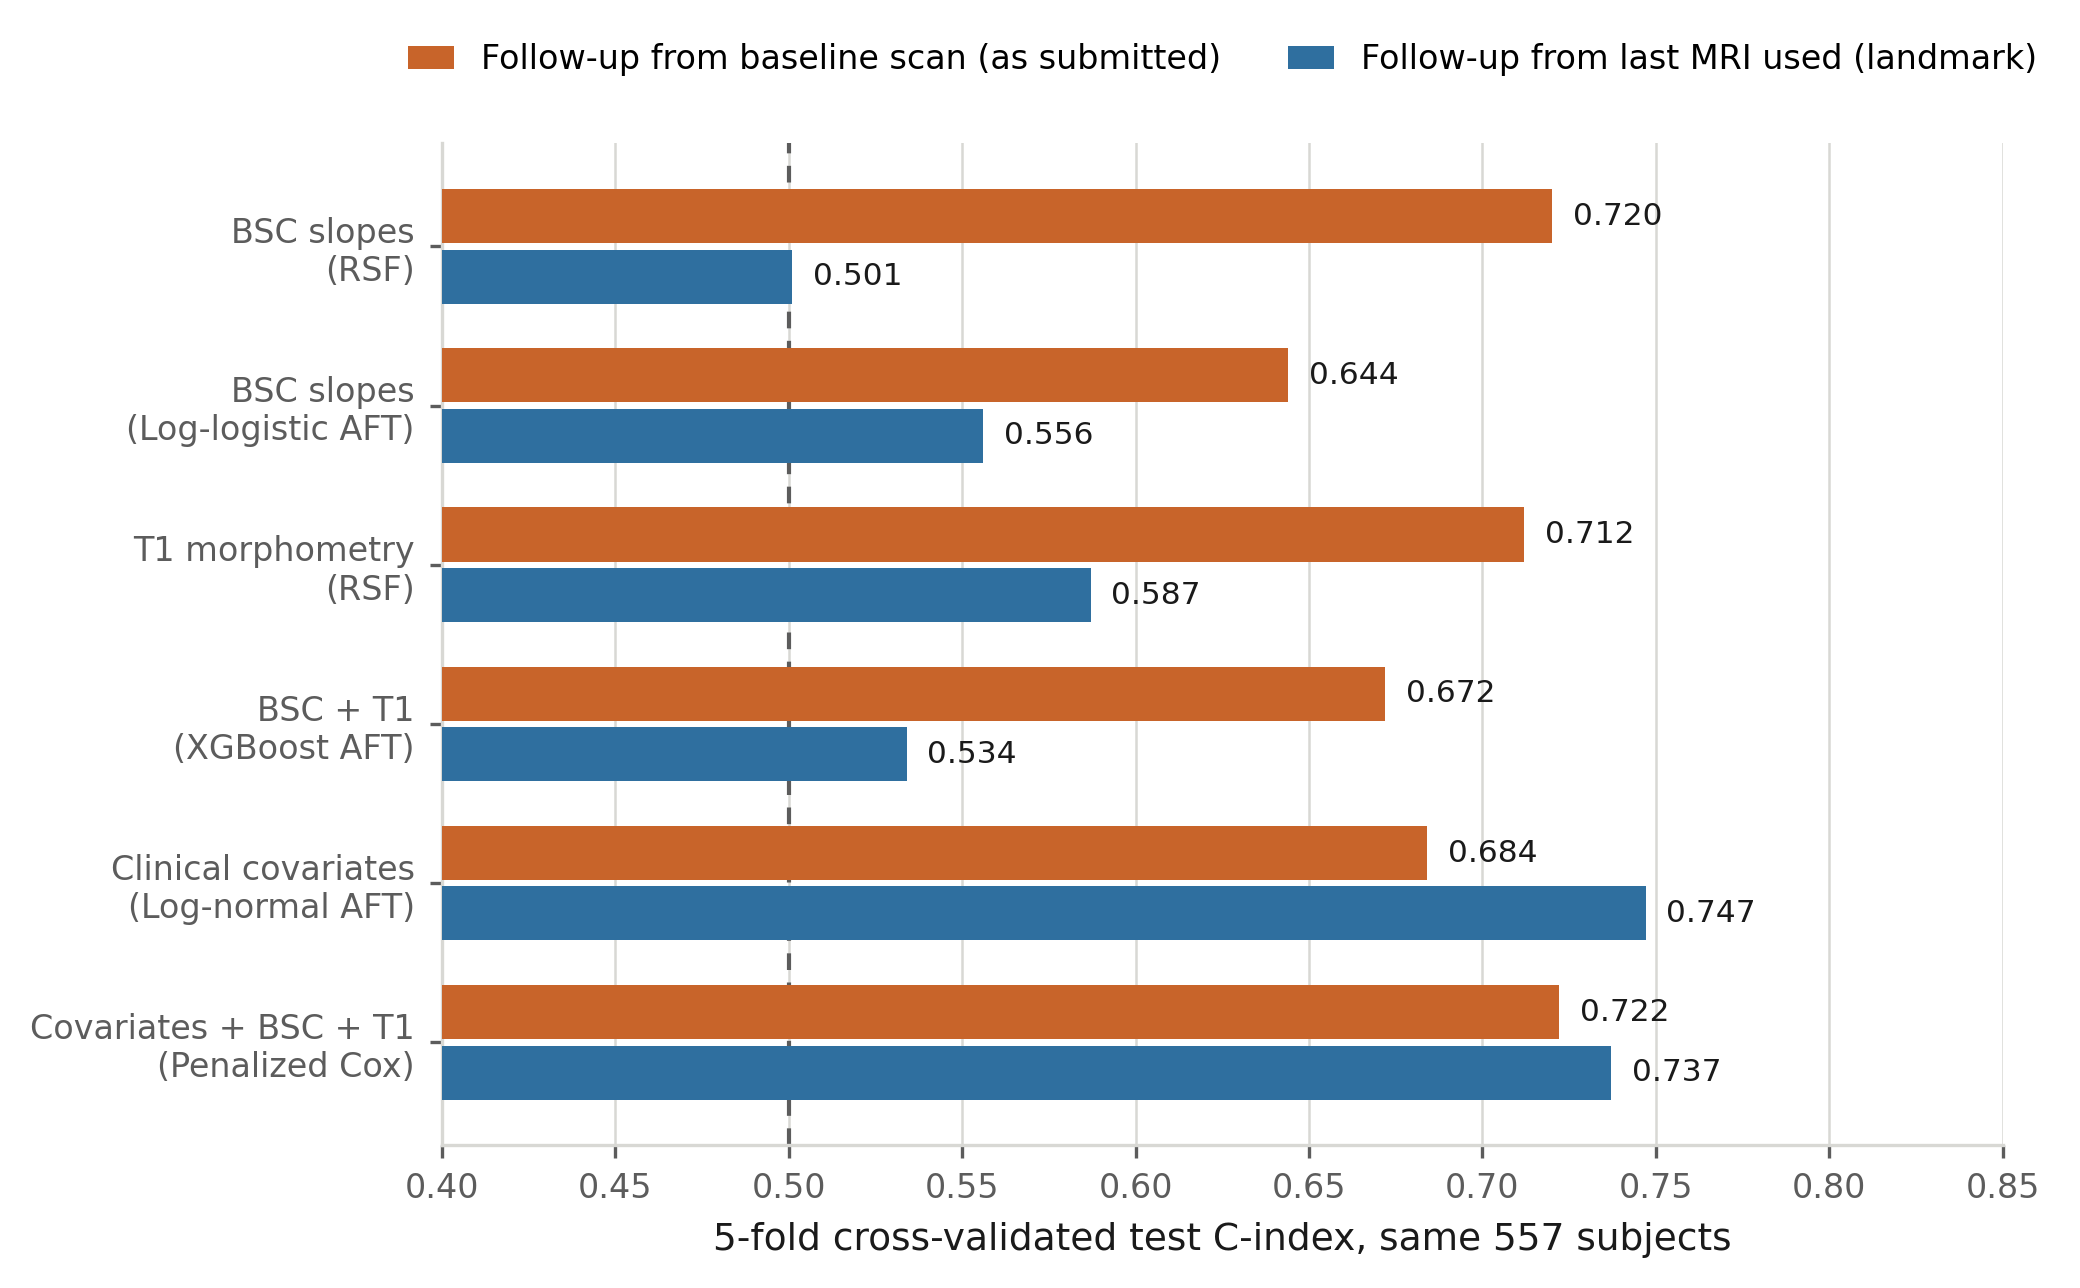
\includegraphics[width=0.86\textwidth]{revision/fig_design_effect.png}
\caption{The same 557 participants, features, folds, hyperparameters and random seed, scored under two definitions of follow-up. Orange bars start the survival clock at the baseline scan while features are drawn from the whole scan series. Blue bars start it at the landmark, with features restricted to scans acquired before it. Imaging blocks lose most of their apparent discrimination; the clinical model gains.}
\label{fig:design}
\end{figure*}

\begin{figure*}[t]
\centering
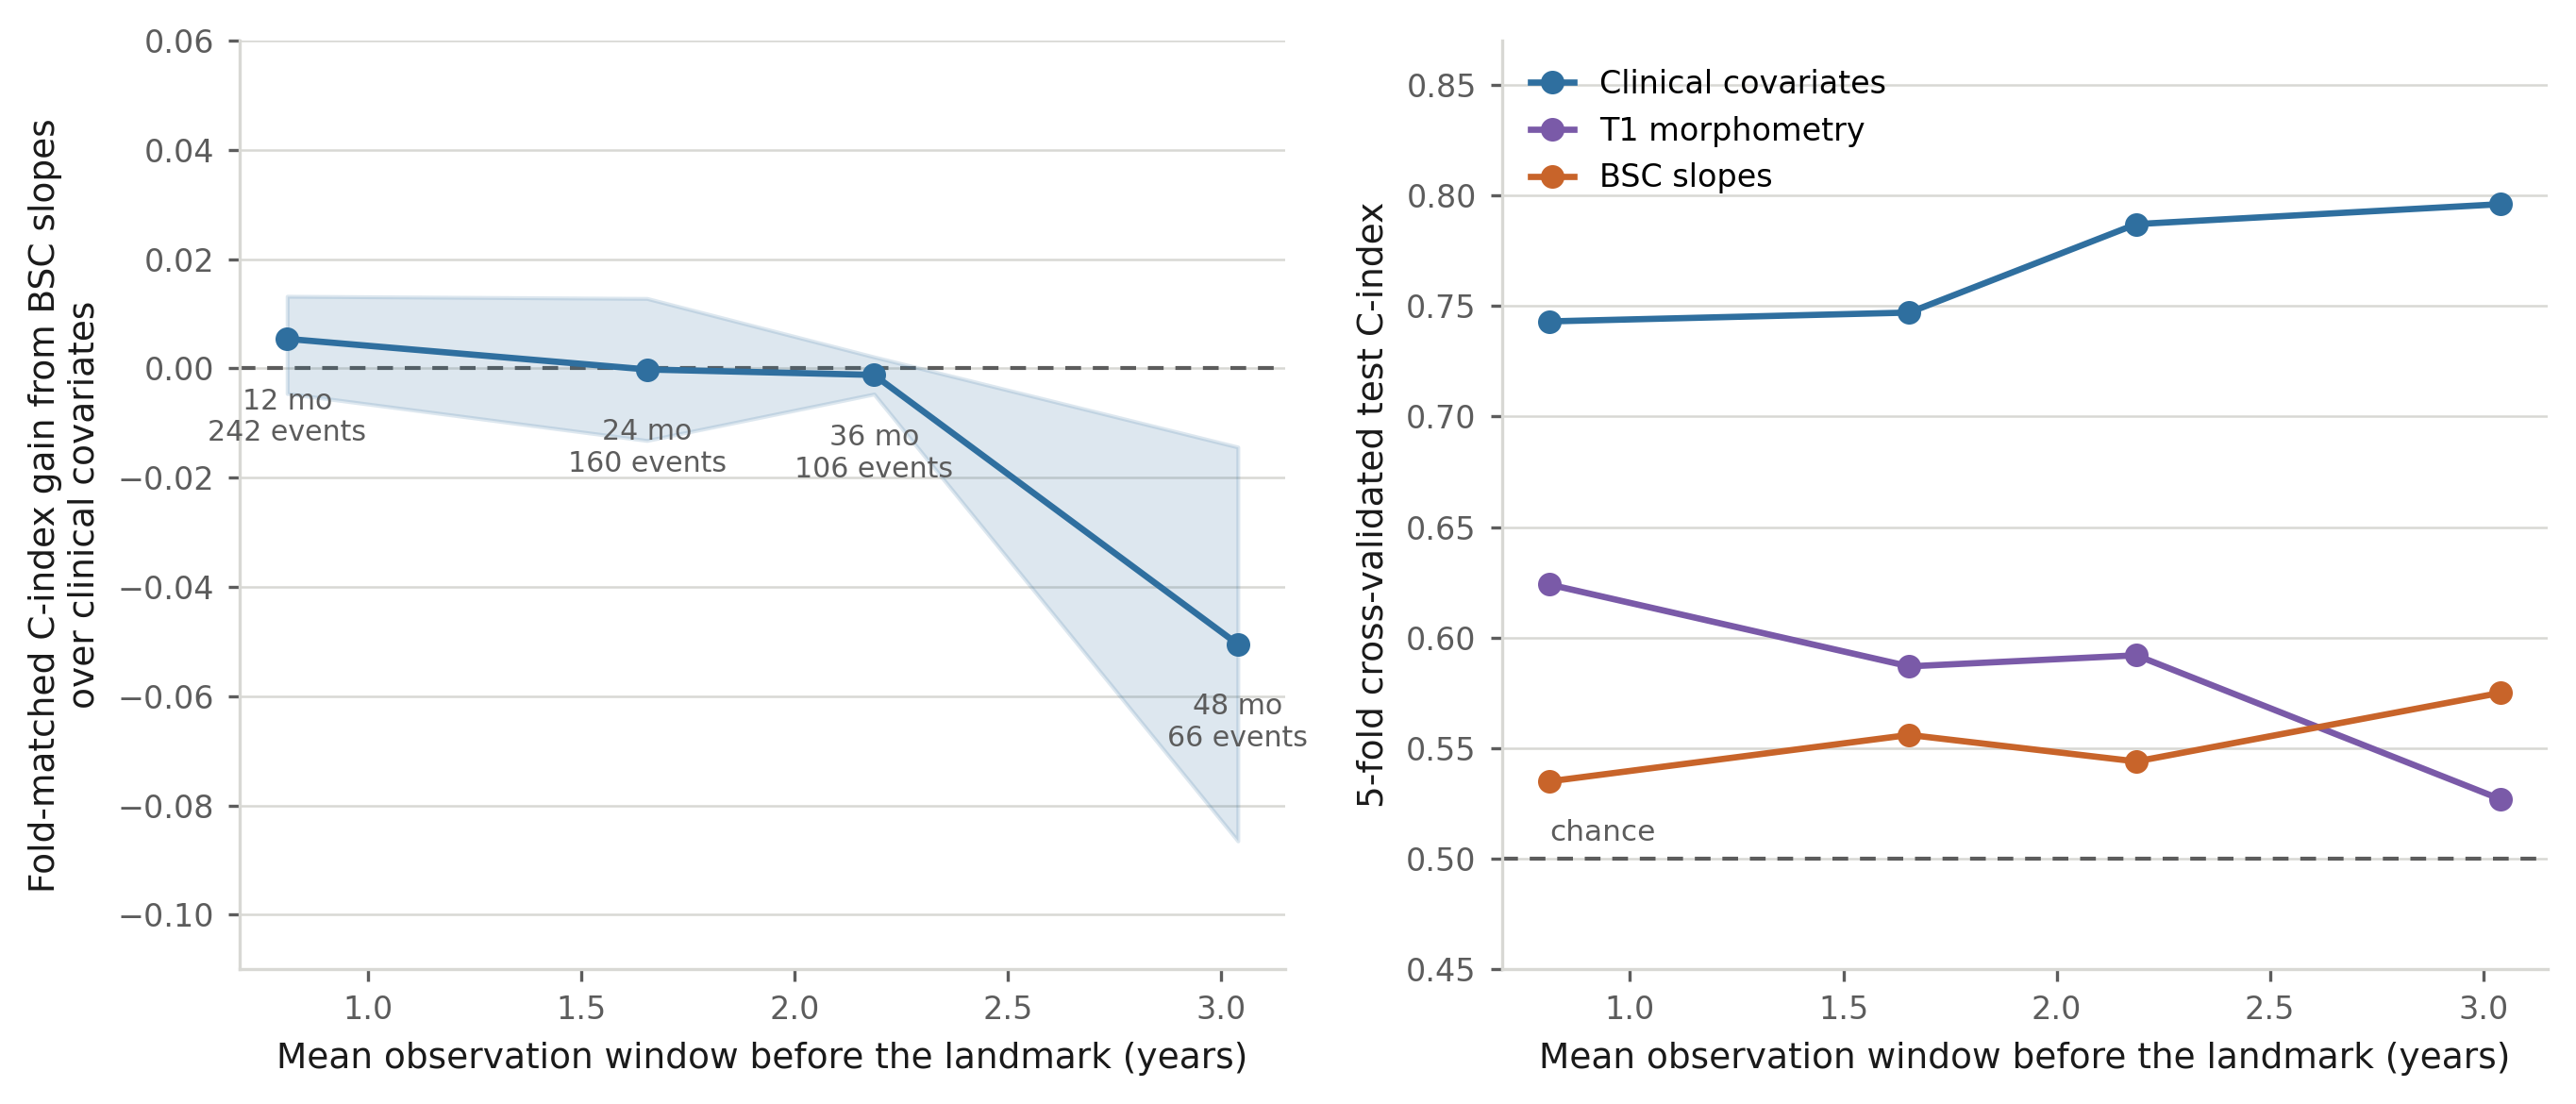
\includegraphics[width=0.96\textwidth]{revision/fig_window_sweep.png}
\caption{Observation-window sweep across landmarks at 12, 24, 36 and 48 months. Left: fold-matched gain in C-index from adding BSC slopes to clinical covariates, with a bootstrap 95\% interval. The mean pre-landmark window quadruples along the x-axis while the gain stays on zero and turns negative at the longest window, where only 66 events remain. Right: discrimination for each feature block. Clinical performance rises as later landmarks select a cohort that is easier to discriminate, while both imaging blocks stay near chance.}
\label{fig:window}
\end{figure*}

\begin{figure*}[t]
\centering
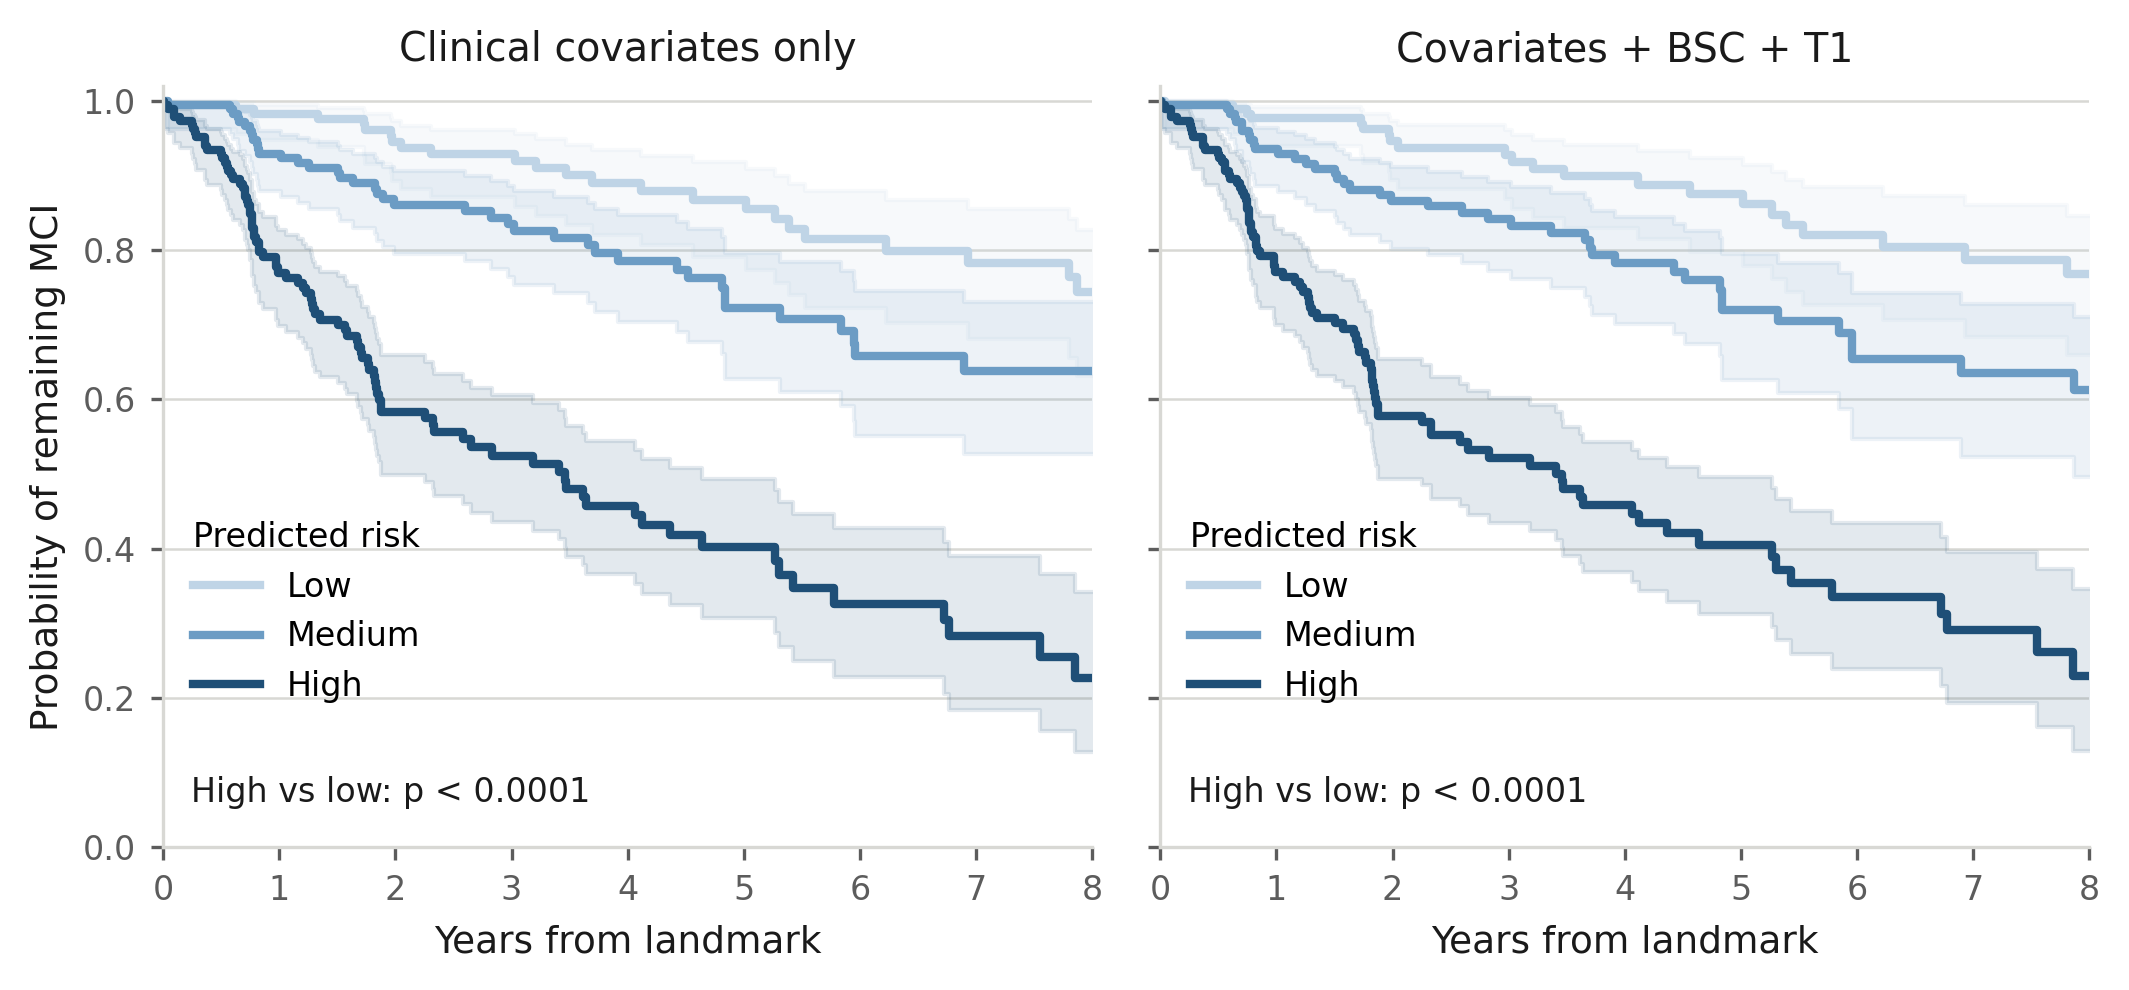
\includegraphics[width=0.86\textwidth]{revision/fig_landmark_km.png}
\caption{Kaplan-Meier curves by predicted-risk tertile at the 24-month landmark, using out-of-fold predictions so every participant is scored by a model that did not see them. Left: clinical covariates. Right: covariates plus both imaging blocks. Adding imaging does not improve separation.}
\label{fig:km}
\end{figure*}

\end{document}
